This chapter introduces baseline results and our results.

\section{Winoground}

\subsection{Compared To Humans}

\subsubsection{Baseline}

We show baseline results in \cref{tab:results_aggr_baseline}, which includes the following multimodal transformers: CLIP \cite{radford2021clip}, FLAVA \cite{singh2022flava}, LXMERT \cite{tan2020lxmert}, UniT \cite{hu2021unit}, UNITER \cite{chen2020uniter}, VILLA \cite{gan2020villa}, VinVL \cite{zhang2021vinvl}, ViLT \cite{kim2021vilt}, VisualBERT \cite{li2019visualbert} and ViLBERT \cite{lu2019vilbert}. They also evaluate several configurations of two types of RNN-based models: VSE++ \cite{faghri2018vse} and VSRN \cite{li2019vsrn}.

\begin{table}[ht]
\centering
\begin{tabular}{l|rrr|rrr}
\toprule
 &
  \multicolumn{3}{c|}{{Score}} &
  \multicolumn{3}{c}{{Accuracy}} \\
 Model                               & Text           & Image          & Group          & Text       & Image      & Group      \\
\midrule
 MTurk Human                         & \textbf{89.50} & \textbf{88.50} & \textbf{85.50} & \textbf{93.75} & \textbf{93.88} & \textbf{93.81} \\
 Random Chance                       & 25.00          & 25.00          & 16.67          & 50.00          & 50.00          & 50.00          \\
 \midrule
 VinVL                        & \textbf{37.75} & 17.75          & 14.50          & \textbf{62.75} & \textbf{57.75} & \textbf{60.25} \\
 UNITER$_{large}$             & \textbf{38.00} & 14.00          & 10.50          & \textbf{63.25} & \textbf{55.75} & \textbf{59.50} \\
 UNITER$_{base}$              & \textbf{32.25} & 13.25          & 10.00          & \textbf{60.62} & \textbf{55.50} & \textbf{58.06} \\
 ViLLA$_{large}$              & \textbf{37.00} & 13.25          & 11.00          & \textbf{62.62} & \textbf{55.25} & \textbf{58.94} \\
 ViLLA$_{base}$               & \textbf{30.00} & 12.00          & 8.00           & \textbf{59.62} & \textbf{55.00} & \textbf{57.31} \\
 VisualBERT$_{base}$          & 15.50          & 2.50           & 1.50           & \textbf{50.50} & 49.88          & \textbf{50.19} \\
 ViLT (ViT-B/32)              & \textbf{34.75} & 14.00          & 9.25           & \textbf{60.50} & \textbf{55.38} & \textbf{57.94} \\
 LXMERT                       & 19.25          & 7.00           & 4.00           & \textbf{52.12} & \textbf{51.88} & \textbf{52.00} \\
 ViLBERT$_{base}$             & 23.75          & 7.25           & 4.75           & \textbf{57.25} & \textbf{52.50} & \textbf{54.87} \\
 UniT$_{ITM Finetuned}$       & 19.50          & 6.25           & 4.00           & \textbf{50.25} & \textbf{50.75} & \textbf{50.50} \\
 FLAVA$_{ITM}$                & \textbf{32.25} & 20.50          & 14.25          & \textbf{62.75} & \textbf{59.13} & \textbf{60.94} \\
 FLAVA$_{Contrastive}$        & \textbf{25.25} & 13.50          & 9.00           & \textbf{59.25} & \textbf{55.12} & \textbf{57.19} \\
 CLIP (ViT-B/32)              & \textbf{30.75} & 10.50          & 8.00           & \textbf{60.38} & \textbf{53.25} & \textbf{56.81} \\
 VSE++$_{COCO}$ (ResNet)      & 22.75          & 8.00           & 4.00           & \textbf{51.38} & \textbf{50.88} & \textbf{51.12} \\
 VSE++$_{COCO}$ (VGG)         & 18.75          & 5.50           & 3.50           & \textbf{50.38} & 49.75          & \textbf{50.06} \\
 VSE++$_{Flickr30k}$ (ResNet) & 20.00          & 5.00           & 2.75           & \textbf{51.50} & \textbf{50.25} & \textbf{50.88} \\
 VSE++$_{Flickr30k}$ (VGG)    & 19.75          & 6.25           & 4.50           & \textbf{52.75} & \textbf{51.00} & \textbf{51.88} \\
 VSRN$_{COCO}$                & 17.50          & 7.00           & 3.75           & \textbf{50.38} & \textbf{51.12} & \textbf{50.75} \\
 VSRN$_{Flickr30k}$           & 20.00          & 5.00           & 3.50           & \textbf{53.25} & \textbf{51.75} & \textbf{52.50} \\
\bottomrule
\end{tabular}
\caption{Results on the Winoground dataset across the text, image and group score and accuracy metrics. Results above random chance in \textbf{bold}.}
\label{tab:results_aggr_baseline}
\end{table}

\subsubsection{Ours}

We show our results in \cref{tab:results_aggr_ours}, which includes various configurations of the following multimodal transformers: OFA \cite{wang2022unifying}, BLIP \cite{li2022blip}, CLIP \cite{radford2021clip}, FLAVA \cite{singh2022flava} and ViLT \cite{kim2021vilt}.

We test 4 different versions of ViLT. The first one is the pre-trained only version, without finetuning. Two others are finetuned for retrieval on COCO and Flickr30k. The last one is finetuned for visual reasoning on NLVR2. The best one is the one trained on NLVR2, which shows that finetuning on that task helps perform better on Winoground. Finetuning for retrieval is also helpful and improves the results of the pre-trained model. The score of the pre-trained model is lower than the baseline one.

For FLAVA and CLIP we manage to replicate baseline results. We also test 3 other CLIP models with different configurations and find that they all perform similar to the baseline configuration.

We test the 5 model sizes of OFA. Taking into account that this model gets state-of-the-art performance on many tasks, the performance is not very good. Even the biggest model is not better than the best baseline model. OFA is trained to generate "yes" or "no" when given an image and the text "Does the image describe <caption>?". This might explain why it does not perform that well on retrieval and Winoground.

We test many configurations of BLIP, which include different training sizes, scoring, vision transformer sizes and finetuning datasets. ITM score is better than ITC score in all the cases. Even the 14M pretrained only model is better than all the previously tested models. Finetuning for retrieval on COCO and Flickr30k improves the results even more, reaching nearly above random performance in text, image and group scores.

However, even the best model is still far from human performance in text, image and group scores. If we look at accuracy metrics, the gap is reduced, but the difference is still very big. Image score remains much lower than text score for all the models.

\begin{table}[ht]
\centering
\begin{tabular}{l|rrr|rrr}
\toprule
 &
  \multicolumn{3}{c|}{{Score}} &
  \multicolumn{3}{c}{{Accuracy}} \\
 Model                               & Text           & Image          & Group          & Text       & Image      & Group      \\
\midrule
 MTurk Human                         & \textbf{89.50} & \textbf{88.50} & \textbf{85.50} & \textbf{93.75} & \textbf{93.88} & \textbf{93.81} \\
 Random Chance                       & 25.00          & 25.00          & 16.67          & 50.00          & 50.00          & 50.00          \\
 \midrule
 ViLT (ViT-B/32)                     & \textbf{27.50} & 8.75           & 6.00           & \textbf{56.88} & \textbf{53.12} & \textbf{55.00} \\
 ViLT$_{COCO}$ (ViT-B/32)            & \textbf{32.75} & 13.50          & 11.25          & \textbf{61.88} & \textbf{56.00} & \textbf{58.94} \\
 ViLT$_{Flickr30k}$ (ViT-B/32)       & \textbf{35.00} & 11.50          & 9.75           & \textbf{61.62} & \textbf{54.50} & \textbf{58.06} \\
 ViLT$_{NLVR2}$ (ViT-B/32)           & \textbf{38.00} & 15.25          & 12.00          & \textbf{58.75} & \textbf{55.62} & \textbf{57.19} \\
 ViLT$_{VSR}$ Random (ViT-B/32)      & \textbf{30.50} & 14.50          & 8.00           & \textbf{59.00} & \textbf{55.75} & \textbf{57.38} \\
 ViLT$_{VSR}$ Zero-shot (ViT-B/32)   & \textbf{29.50} & 14.00          & 9.25           & \textbf{58.38} & \textbf{54.75} & \textbf{56.56} \\
 FLAVA$_{ITM}$                       & \textbf{32.25} & 20.50          & 14.25          & \textbf{62.75} & \textbf{59.13} & \textbf{60.94} \\
 FLAVA$_{ITC}$                       & \textbf{25.25} & 13.50          & 9.00           & \textbf{59.25} & \textbf{55.12} & \textbf{57.19} \\
 CLIP (ViT-B/32)                     & \textbf{30.75} & 10.25          & 8.25           & \textbf{60.38} & \textbf{53.12} & \textbf{56.75} \\
 CLIP (ViT-B/16)                     & 25.00          & 10.25          & 7.00           & \textbf{57.88} & \textbf{53.75} & \textbf{55.81} \\
 CLIP (ViT-L/14)                     & \textbf{28.50} & 11.00          & 8.00           & \textbf{60.38} & \textbf{54.62} & \textbf{57.50} \\
 CLIP (ViT-L/14-336)                 & \textbf{27.50} & 12.00          & 8.00           & \textbf{59.38} & \textbf{55.12} & \textbf{57.25} \\
 OFA$_{Tiny}$                        & 20.50          & 8.00           & 3.75           & \textbf{53.50} & \textbf{52.00} & \textbf{52.75} \\
 OFA$_{Base}$                        & \textbf{26.50} & 10.50          & 7.00           & \textbf{58.88} & \textbf{54.00} & \textbf{56.44} \\
 OFA$_{Medium}$                      & 22.75          & 9.00           & 5.50           & \textbf{54.25} & \textbf{52.75} & \textbf{53.50} \\
 OFA$_{Large}$                       & \textbf{26.00} & 8.75           & 5.75           & \textbf{58.38} & \textbf{52.88} & \textbf{55.62} \\
 OFA$_{Huge}$                        & \textbf{36.25} & 15.50          & 13.50          & \textbf{64.38} & \textbf{56.62} & \textbf{60.50} \\
 BLIP$_{ITM 14M}$ (ViT-B/16)         & \textbf{39.25} & 19.00          & 15.00          & \textbf{65.88} & \textbf{58.25} & \textbf{62.06} \\
 BLIP$_{ITC 14M}$ (ViT-B/16)         & \textbf{32.25} & 13.75          & 10.50          & \textbf{62.25} & \textbf{56.50} & \textbf{59.38} \\
 BLIP$_{ITM}$ (ViT-B/16)             & \textbf{40.50} & 20.50          & 16.50          & \textbf{66.25} & \textbf{59.00} & \textbf{62.62} \\
 BLIP$_{ITC}$ (ViT-B/16)             & \textbf{29.75} & 14.50          & 9.50           & \textbf{59.88} & \textbf{56.12} & \textbf{58.00} \\
 BLIP$_{ITM}$ (ViT-B/16) (CapFilt-L) & \textbf{37.50} & 18.50          & 14.00          & \textbf{65.00} & \textbf{59.13} & \textbf{62.06} \\
 BLIP$_{ITC}$ (ViT-B/16) (CapFilt-L) & \textbf{31.50} & 10.50          & 8.50           & \textbf{61.38} & \textbf{53.62} & \textbf{57.50} \\
 BLIP$_{ITM}$ (ViT-L/16)             & \textbf{42.50} & 18.25          & 15.50          & \textbf{66.88} & \textbf{57.25} & \textbf{62.06} \\
 BLIP$_{ITC}$ (ViT-L/16)             & \textbf{33.25} & 12.00          & 9.00           & \textbf{61.75} & \textbf{55.00} & \textbf{58.38} \\
 BLIP$_{ITM COCO}$ (ViT-B/16)        & \textbf{48.00} & 24.50          & \textbf{20.00} & \textbf{69.88} & \textbf{61.25} & \textbf{65.56} \\
 BLIP$_{ITC COCO}$ (ViT-B/16)        & \textbf{37.75} & 15.75          & 12.75          & \textbf{65.00} & \textbf{56.88} & \textbf{60.94} \\
 BLIP$_{ITM Flickr30k}$ (ViT-B/16)   & \textbf{46.25} & 24.25          & \textbf{21.25} & \textbf{69.25} & \textbf{60.62} & \textbf{64.94} \\
 BLIP$_{ITC Flickr30k}$ (ViT-B/16)   & \textbf{38.25} & 15.00          & 12.25          & \textbf{65.38} & \textbf{56.12} & \textbf{60.75} \\
 BLIP$_{ITM COCO}$ (ViT-L/16)        & \textbf{46.75} & 24.00          & \textbf{20.50} & \textbf{68.88} & \textbf{61.00} & \textbf{64.94} \\
 BLIP$_{ITC COCO}$ (ViT-L/16)        & \textbf{37.75} & 13.75          & 10.50          & \textbf{64.88} & \textbf{55.75} & \textbf{60.31} \\
 BLIP$_{ITM Flickr30k}$ (ViT-L/16)   & \textbf{45.00} & 24.75          & \textbf{20.50} & \textbf{68.62} & \textbf{60.50} & \textbf{64.56} \\
 BLIP$_{ITC Flickr30k}$ (ViT-L/16)   & \textbf{36.00} & 16.25          & 13.50          & \textbf{63.38} & \textbf{56.75} & \textbf{60.06} \\
 BLIP$_{NLVR2}$ (ViT-B/16)           & \textbf{40.25} & 25.00          & \textbf{18.50} & \textbf{64.62} & \textbf{61.62} & \textbf{63.12} \\
\bottomrule
\end{tabular}
\caption{Results on the Winoground dataset across the text, image and group score and accuracy metrics. Results above random chance in \textbf{bold}.}
\label{tab:results_aggr_ours}
\end{table}

\subsection{Results By Linguistic Tag}

\subsubsection{Baseline}

See \cref{tab:results-by-ling-tag-baseline}

\begin{table}[ht]
    \centering
    \begin{adjustbox}{max width=\textwidth}
  \begin{tabular}{l|rrr|rrr|rrr|rrr|rrr}
    \toprule
     &
      \multicolumn{3}{c|}{Object} &
      \multicolumn{3}{c|}{Relation} &
      \multicolumn{3}{c|}{Both} &
      \multicolumn{3}{c|}{1 Main Pred} &
      \multicolumn{3}{c}{2 Main Preds}\\
    Model & Text & Image & Group & Text & Image & Group & Text & Image & Group & Text & Image & Group & Text & Image & Group \\\midrule
 MTurk Human                  & \textbf{92.20} & \textbf{90.78} & \textbf{88.65} & \textbf{89.27} & \textbf{90.56} & \textbf{86.70} & \textbf{76.92} & \textbf{57.69} & \textbf{57.69} & \textbf{87.33} & \textbf{85.62} & \textbf{82.53} & \textbf{95.37} & \textbf{96.30} & \textbf{93.52} \\
 VinVL                        & \textbf{36.88} & 17.73          & 14.18          & \textbf{37.77} & 17.60          & 14.16          & \textbf{42.31} & 19.23          & \textbf{19.23} & \textbf{39.38} & 21.23          & \textbf{17.47} & \textbf{33.33} & 8.33           & 6.48           \\
 UNITER$_{large}$             & \textbf{39.01} & 12.77          & 9.93           & \textbf{36.05} & 14.16          & 9.87           & \textbf{50.00} & 19.23          & \textbf{19.23} & \textbf{40.07} & 16.44          & 13.36          & \textbf{32.41} & 7.41           & 2.78           \\
 UNITER$_{base}$              & \textbf{34.04} & 11.35          & 9.22           & \textbf{30.04} & 14.16          & 10.30          & \textbf{42.31} & 15.38          & 11.54          & \textbf{35.27} & 14.73          & 11.99          & 24.07          & 9.26           & 4.63           \\
 ViLLA$_{large}$              & \textbf{36.88} & 14.89          & 11.35          & \textbf{37.34} & 12.88          & 11.16          & \textbf{34.62} & 7.69           & 7.69           & \textbf{39.73} & 17.12          & 14.38          & \textbf{29.63} & 2.78           & 1.85           \\
 ViLLA$_{base}$               & \textbf{33.33} & 15.60          & 9.93           & \textbf{27.04} & 9.01           & 6.01           & \textbf{38.46} & 19.23          & 15.38          & \textbf{33.22} & 14.04          & 10.27          & 21.30          & 6.48           & 1.85           \\
 VisualBERT$_{base}$          & 19.15          & 2.13           & 0.71           & 12.88          & 2.15           & 1.72           & 19.23          & 7.69           & 3.85           & 16.44          & 2.74           & 1.71           & 12.96          & 1.85           & 0.93           \\
 ViLT (ViT-B/32)              & \textbf{31.91} & 15.60          & 9.22           & \textbf{36.91} & 11.59          & 8.15           & \textbf{30.77} & \textbf{26.92} & \textbf{19.23} & \textbf{35.27} & 17.12          & 11.64          & \textbf{33.33} & 5.56           & 2.78           \\
 LXMERT                       & 22.70          & 9.22           & 6.38           & 17.60          & 5.58           & 2.58           & 15.38          & 7.69           & 3.85           & 19.18          & 8.56           & 5.14           & 19.44          & 2.78           & 0.93           \\
 ViLBERT$_{base}$             & \textbf{29.08} & 10.64          & 7.09           & 19.31          & 3.00           & 1.72           & \textbf{34.62} & \textbf{26.92} & \textbf{19.23} & 23.97          & 8.90           & 5.82           & 23.15          & 2.78           & 1.85           \\
 UniT$_{ITM finetuned}$       & 17.73          & 5.67           & 2.13           & 18.03          & 4.72           & 3.43           & \textbf{42.31} & 23.08          & \textbf{19.23} & 21.58          & 6.85           & 4.11           & 13.89          & 4.63           & 3.70           \\
  FLAVA$_{ITM}$                & \textbf{31.91} & 23.40 & 14.89 & \textbf{30.04} & 16.31 & 12.02 & \textbf{53.85} & \textbf{42.31} & \textbf{30.77} & \textbf{36.30} & 24.66 & \textbf{17.81} & 21.30          & 9.26 & 4.63 \\
 FLAVA$_{Contrastive}$        & 23.40          & 19.15 & 11.35 & 23.61          &  8.58 &  5.58 & \textbf{50.00} & \textbf{26.92} & \textbf{26.92} & \textbf{26.37} & 16.44 & 10.62          & 22.22          &  5.56 & 4.63 \\
 CLIP (ViT-B/32)              & \textbf{34.75} & 7.80           & 6.38           & 22.75          & 8.58           & 5.58           & \textbf{80.77} & \textbf{42.31} & \textbf{38.46} & \textbf{35.27} & 13.01          & 10.27          & 18.52          & 3.70           & 1.85           \\
 VSE++$_{COCO}$ (ResNet)      & 21.99          & 6.38           & 1.42           & 23.61          & 9.01           & 5.58           & 19.23          & 7.69           & 3.85           & 25.00          & 9.59           & 4.79           & 16.67          & 3.70           & 1.85           \\
 VSE++$_{COCO}$ (VGG)         & 17.73          & 2.13           & 2.13           & 18.45          & 7.30           & 3.86           & \textbf{26.92} & 7.69           & 7.69           & 18.49          & 4.79           & 2.74           & 19.44          & 7.41           & 5.56           \\
 VSE++$_{Flickr30k}$ (ResNet) & 20.57          & 6.38           & 3.55           & 18.88          & 4.29           & 2.15           & \textbf{26.92} & 3.85           & 3.85           & 21.58          & 6.51           & 3.42           & 15.74          & 0.93           & 0.93           \\
 VSE++$_{Flickr30k}$ (VGG)    & 17.73          & 4.96           & 2.84           & 19.74          & 6.87           & 5.15           & \textbf{30.77} & 7.69           & 7.69           & 20.55          & 6.16           & 4.79           & 17.59          & 6.48           & 3.70           \\
 VSRN$_{COCO}$                & 15.60          & 4.96           & 2.13           & 18.88          & 7.73           & 4.72           & 15.38          & 11.54          & 3.85           & 17.12          & 7.19           & 3.77           & 18.52          & 6.48           & 3.70           \\
 VSRN$_{Flickr30k}$           & 16.31          & 4.96           & 2.13           & 21.03          & 4.29           & 3.86           & \textbf{30.77} & 11.54          & 7.69           & 20.89          & 5.82           & 3.77           & 17.59          & 2.78           & 2.78           \\
          \bottomrule
  \end{tabular}
  \end{adjustbox}
  \caption{The results by linguistic tag. Results above chance are in \textbf{bold}.}
    \label{tab:results-by-ling-tag-baseline}
\end{table}

\subsubsection{Ours}

See \cref{tab:results-by-ling-tag-ours}

\begin{table}[ht]
    \centering
    \begin{adjustbox}{max width=\textwidth}
  \begin{tabular}{l|rrr|rrr|rrr|rrr|rrr}
    \toprule
     &
      \multicolumn{3}{c|}{Object} &
      \multicolumn{3}{c|}{Relation} &
      \multicolumn{3}{c|}{Both} &
      \multicolumn{3}{c|}{1 Main Pred} &
      \multicolumn{3}{c}{2 Main Preds}\\
    Model & Text & Image & Group & Text & Image & Group & Text & Image & Group & Text & Image & Group & Text & Image & Group \\\midrule
 MTurk Human                  & \textbf{92.20} & \textbf{90.78} & \textbf{88.65} & \textbf{89.27} & \textbf{90.56} & \textbf{86.70} & \textbf{76.92} & \textbf{57.69} & \textbf{57.69} & \textbf{87.33} & \textbf{85.62} & \textbf{82.53} & \textbf{95.37} & \textbf{96.30} & \textbf{93.52} \\
 ViLT (ViT-B/32)                     & \textbf{29.08} & 10.64          & 4.96           & \textbf{26.18} & 7.73           & 6.44           & \textbf{30.77} & 7.69           & 7.69           & \textbf{30.14} & 10.62          & 7.53           & 20.37          & 3.70           & 1.85           \\
 ViLT$_{COCO}$ (ViT-B/32)            & \textbf{33.33} & 15.60          & 12.77          & \textbf{30.90} & 10.73          & 9.01           & \textbf{46.15} & \textbf{26.92} & \textbf{23.08} & \textbf{36.64} & 15.75          & 14.04          & 22.22          & 7.41           & 3.70           \\
 ViLT$_{Flickr30k}$ (ViT-B/32)       & \textbf{32.62} & 14.89          & 11.35          & \textbf{35.62} & 8.15           & 7.73           & \textbf{42.31} & 23.08          & \textbf{19.23} & \textbf{36.99} & 14.38          & 11.99          & \textbf{29.63} & 3.70           & 3.70           \\
 ViLT$_{NLVR2}$ (ViT-B/32)           & \textbf{39.01} & 16.31          & 14.18          & \textbf{36.48} & 14.59          & 10.30          & \textbf{46.15} & 15.38          & 15.38          & \textbf{39.73} & 18.15          & 15.07          & \textbf{33.33} & 7.41           & 3.70           \\
 ViLT$_{VSR}$ Random (ViT-B/32)      & \textbf{34.75} & 17.73          & 9.93           & \textbf{27.47} & 11.16          & 6.01           & \textbf{34.62} & \textbf{26.92} & 15.38          & \textbf{32.53} & 16.44          & 9.59           & 25.00          & 9.26           & 3.70           \\
 ViLT$_{VSR}$ Zero-shot (ViT-B/32)   & \textbf{34.75} & 19.86          & 14.18          & \textbf{26.18} & 10.73          & 6.44           & \textbf{30.77} & 11.54          & 7.69           & \textbf{32.19} & 15.75          & 11.30          & 22.22          & 9.26           & 3.70           \\
 FLAVA$_{ITM}$                       & \textbf{31.91} & 23.40          & 14.89          & \textbf{30.04} & 16.31          & 12.02          & \textbf{53.85} & \textbf{42.31} & \textbf{30.77} & \textbf{36.30} & 24.66          & \textbf{17.81} & 21.30          & 9.26           & 4.63           \\
 FLAVA$_{ITC}$                       & 23.40          & 19.15          & 11.35          & 23.61          & 8.58           & 5.58           & \textbf{50.00} & \textbf{26.92} & \textbf{26.92} & \textbf{26.37} & 16.44          & 10.62          & 22.22          & 5.56           & 4.63           \\
 CLIP (ViT-B/32)                     & \textbf{35.46} & 7.80           & 6.38           & 22.32          & 7.73           & 5.58           & \textbf{80.77} & \textbf{46.15} & \textbf{42.31} & \textbf{35.62} & 13.01          & 10.62          & 17.59          & 2.78           & 1.85           \\
 CLIP (ViT-B/16)                     & \textbf{27.66} & 10.64          & 5.67           & 19.31          & 6.44           & 4.29           & \textbf{61.54} & \textbf{42.31} & \textbf{38.46} & \textbf{30.14} & 11.99          & 8.90           & 11.11          & 5.56           & 1.85           \\
 CLIP (ViT-L/14)                     & \textbf{27.66} & 8.51           & 5.67           & \textbf{25.75} & 9.87           & 6.44           & \textbf{57.69} & \textbf{34.62} & \textbf{34.62} & \textbf{30.14} & 13.01          & 9.93           & 24.07          & 5.56           & 2.78           \\
 CLIP (ViT-L/14-336)                 & \textbf{32.62} & 12.77          & 9.22           & 21.03          & 8.15           & 4.29           & \textbf{57.69} & \textbf{42.31} & \textbf{34.62} & \textbf{30.48} & 14.04          & 10.62          & 19.44          & 6.48           & 0.93           \\
 OFA$_{Tiny}$                        & 22.70          & 6.38           & 2.13           & 17.17          & 6.87           & 3.43           & \textbf{38.46} & \textbf{26.92} & 15.38          & 23.97          & 8.22           & 4.45           & 11.11          & 7.41           & 1.85           \\
 OFA$_{Base}$                        & \textbf{25.53} & 14.18          & 7.09           & 24.46          & 6.87           & 5.15           & \textbf{50.00} & 23.08          & \textbf{23.08} & \textbf{28.77} & 12.67          & 8.56           & 20.37          & 4.63           & 2.78           \\
 OFA$_{Medium}$                      & 19.86          & 7.80           & 4.26           & 22.32          & 7.73           & 4.72           & \textbf{42.31} & \textbf{26.92} & \textbf{19.23} & 24.32          & 10.96          & 6.85           & 18.52          & 3.70           & 1.85           \\
 OFA$_{Large}$                       & \textbf{26.24} & 10.64          & 5.67           & 24.03          & 5.15           & 3.86           & \textbf{42.31} & \textbf{30.77} & \textbf{23.08} & \textbf{29.45} & 10.96          & 7.53           & 16.67          & 2.78           & 0.93           \\
 OFA$_{Huge}$                        & \textbf{40.43} & 18.44          & 15.60          & \textbf{30.90} & 11.59          & 9.87           & \textbf{61.54} & \textbf{34.62} & \textbf{34.62} & \textbf{39.73} & 19.18          & \textbf{16.78} & \textbf{26.85} & 5.56           & 4.63           \\
 BLIP$_{ITM 14M}$ (ViT-B/16)         & \textbf{41.84} & 23.40          & \textbf{17.73} & \textbf{36.05} & 14.59          & 11.59          & \textbf{53.85} & \textbf{34.62} & \textbf{30.77} & \textbf{43.84} & 23.63          & \textbf{18.49} & \textbf{26.85} & 6.48           & 5.56           \\
 BLIP$_{ITC 14M}$ (ViT-B/16)         & \textbf{34.04} & 13.48          & 9.93           & \textbf{28.33} & 12.02          & 9.44           & \textbf{57.69} & \textbf{30.77} & \textbf{23.08} & \textbf{37.67} & 16.44          & 13.01          & 17.59          & 6.48           & 3.70           \\
 BLIP$_{ITM}$ (ViT-B/16)             & \textbf{46.10} & 22.70          & \textbf{17.73} & \textbf{35.62} & 17.60          & 14.16          & \textbf{53.85} & \textbf{34.62} & \textbf{30.77} & \textbf{45.89} & \textbf{25.34} & \textbf{20.55} & \textbf{25.93} & 7.41           & 5.56           \\
 BLIP$_{ITC}$ (ViT-B/16)             & \textbf{34.75} & 14.18          & 9.22           & \textbf{25.32} & 13.73          & 8.58           & \textbf{42.31} & 23.08          & \textbf{19.23} & \textbf{33.56} & 16.10          & 10.62          & 19.44          & 10.19          & 6.48           \\
 BLIP$_{ITM}$ (ViT-B/16) (CapFilt-L) & \textbf{39.01} & 19.86          & 12.77          & \textbf{34.76} & 15.88          & 12.45          & \textbf{53.85} & \textbf{34.62} & \textbf{34.62} & \textbf{41.10} & 22.60          & \textbf{17.12} & \textbf{27.78} & 7.41           & 5.56           \\
 BLIP$_{ITC}$ (ViT-B/16) (CapFilt-L) & \textbf{36.88} & 12.77          & 9.22           & \textbf{26.18} & 8.58           & 7.30           & \textbf{50.00} & 15.38          & 15.38          & \textbf{35.96} & 13.36          & 10.96          & 19.44          & 2.78           & 1.85           \\
 BLIP$_{ITM}$ (ViT-L/16)             & \textbf{41.84} & 19.86          & \textbf{17.02} & \textbf{40.77} & 16.31          & 13.73          & \textbf{61.54} & \textbf{26.92} & \textbf{23.08} & \textbf{45.55} & 23.29          & \textbf{20.21} & \textbf{34.26} & 4.63           & 2.78           \\
 BLIP$_{ITC}$ (ViT-L/16)             & \textbf{34.04} & 14.18          & 11.35          & \textbf{30.90} & 9.01           & 6.01           & \textbf{50.00} & \textbf{26.92} & \textbf{23.08} & \textbf{36.99} & 14.04          & 10.96          & 23.15          & 6.48           & 3.70           \\
 BLIP$_{ITM COCO}$ (ViT-B/16)        & \textbf{42.55} & \textbf{26.95} & \textbf{19.15} & \textbf{49.79} & 21.89          & \textbf{19.31} & \textbf{61.54} & \textbf{34.62} & \textbf{30.77} & \textbf{48.97} & \textbf{29.79} & \textbf{24.66} & \textbf{45.37} & 10.19          & 7.41           \\
 BLIP$_{ITC COCO}$ (ViT-B/16)        & \textbf{36.88} & 19.15          & 14.18          & \textbf{36.05} & 11.59          & 10.30          & \textbf{57.69} & \textbf{34.62} & \textbf{26.92} & \textbf{41.78} & 18.84          & 15.07          & \textbf{26.85} & 7.41           & 6.48           \\
 BLIP$_{ITM Flickr30k}$ (ViT-B/16)   & \textbf{49.65} & \textbf{28.37} & \textbf{22.70} & \textbf{42.49} & 19.74          & \textbf{18.45} & \textbf{61.54} & \textbf{42.31} & \textbf{38.46} & \textbf{51.03} & \textbf{28.42} & \textbf{26.03} & \textbf{33.33} & 12.96          & 8.33           \\
 BLIP$_{ITC Flickr30k}$ (ViT-B/16)   & \textbf{36.88} & 17.02          & 10.64          & \textbf{36.48} & 12.02          & 11.16          & \textbf{61.54} & \textbf{30.77} & \textbf{30.77} & \textbf{40.75} & 17.12          & 13.70          & \textbf{31.48} & 9.26           & 8.33           \\
 BLIP$_{ITM COCO}$ (ViT-L/16)        & \textbf{48.94} & \textbf{25.53} & \textbf{20.57} & \textbf{44.64} & 22.32          & \textbf{20.60} & \textbf{53.85} & \textbf{30.77} & \textbf{19.23} & \textbf{51.03} & \textbf{28.42} & \textbf{23.97} & \textbf{35.19} & 12.04          & 11.11          \\
 BLIP$_{ITC COCO}$ (ViT-L/16)        & \textbf{36.88} & 14.18          & 11.35          & \textbf{36.05} & 11.16          & 7.30           & \textbf{57.69} & \textbf{34.62} & \textbf{34.62} & \textbf{41.10} & 16.44          & 13.36          & \textbf{28.70} & 6.48           & 2.78           \\
 BLIP$_{ITM Flickr30k}$ (ViT-L/16)   & \textbf{46.10} & 22.70          & 16.31          & \textbf{42.06} & 24.89          & \textbf{21.46} & \textbf{65.38} & \textbf{34.62} & \textbf{34.62} & \textbf{50.34} & \textbf{29.11} & \textbf{24.66} & \textbf{30.56} & 12.96          & 9.26           \\
 BLIP$_{ITC Flickr30k}$ (ViT-L/16)   & \textbf{39.01} & 19.86          & 15.60          & \textbf{30.47} & 11.59          & 9.44           & \textbf{69.23} & \textbf{38.46} & \textbf{38.46} & \textbf{39.38} & 20.55          & \textbf{17.12} & \textbf{26.85} & 4.63           & 3.70           \\
 BLIP$_{NLVR2}$ (ViT-B/16)           & \textbf{42.55} & 23.40          & \textbf{19.86} & \textbf{36.48} & \textbf{25.32} & \textbf{16.74} & \textbf{61.54} & \textbf{30.77} & \textbf{26.92} & \textbf{42.47} & \textbf{27.74} & \textbf{21.23} & \textbf{34.26} & 17.59          & 11.11    \\
          \bottomrule
  \end{tabular}
  \end{adjustbox}
  \caption{The results by linguistic tag. Results above chance are in \textbf{bold}.}
    \label{tab:results-by-ling-tag-ours}
\end{table}

\subsection{Results By Visual Tag}

\subsubsection{Baseline}

See \cref{tab:results-by-visual-tag-baseline}

\begin{table}[ht]
    \centering
   \begin{adjustbox}{max width=\textwidth}
  \begin{tabular}{l|rrr|rrr|rrr}
    \toprule
     &
      \multicolumn{3}{c|}{Symbolic} &
      \multicolumn{3}{c|}{Pragmatics} &
      \multicolumn{3}{c}{Same Image Series} \\
    Model & Text & Image & Group & Text & Image & Group & Text & Image & Group \\\midrule
 MTurk Human                  & \textbf{96.43} & \textbf{92.86} & \textbf{92.86} & \textbf{58.82} & \textbf{41.18} & \textbf{41.18} & \textbf{95.65} & \textbf{91.30} & \textbf{91.30} \\
 VinVL                        & 25.00          & 17.86          & 14.29          & \textbf{29.41} & 5.88           & 5.88           & \textbf{34.78} & 17.39          & 13.04          \\
 UNITER$_{large}$             & \textbf{39.29} & \textbf{28.57} & \textbf{17.86} & \textbf{35.29} & 0.00           & 0.00           & 4.35           & 8.70           & 0.00           \\
 UNITER$_{base}$              & \textbf{46.43} & 14.29          & 14.29          & \textbf{29.41} & 17.65          & 11.76          & 8.70           & 8.70           & 0.00           \\
 ViLLA$_{large}$              & \textbf{39.29} & 14.29          & 10.71          & 17.65          & 0.00           & 0.00           & 17.39          & 4.35           & 0.00           \\
 ViLLA$_{base}$               & \textbf{42.86} & 17.86          & 14.29          & \textbf{29.41} & 5.88           & 5.88           & 13.04          & 8.70           & 4.35           \\
 VisualBERT$_{base}$          & \textbf{28.57} & 0.00           & 0.00           & 5.88           & 0.00           & 0.00           & 13.04          & 0.00           & 0.00           \\
 ViLT (ViT-B/32)              & \textbf{28.57} & 17.86          & 10.71          & \textbf{35.29} & 0.00           & 0.00           & \textbf{26.09} & 0.00           & 0.00           \\
 LXMERT                       & \textbf{28.57} & 3.57           & 3.57           & 17.65          & 5.88           & 0.00           & 8.70           & 4.35           & 0.00           \\
 ViLBERT$_{base}$             & \textbf{28.57} & 10.71          & 7.14           & \textbf{29.41} & 5.88           & 5.88           & 13.04          & 0.00           & 0.00           \\
 UniT$_{ITM finetuned}$       & 14.29          & 10.71          & 7.14           & 17.65          & 5.88           & 5.88           & 21.74          & 4.35           & 4.35           \\
 FLAVA$_{ITM}$                & 25.00          & \textbf{28.57} & \textbf{17.86} & 17.65          & \textbf{29.41} & 11.76 & 17.39          &  8.70 &  0.00 \\
 FLAVA$_{Contrastive}$        & 17.86          & 10.71          & 10.71          & 11.76          & 23.53          & 5.88           & 17.39          & 4.35           &  4.35 \\
 CLIP (ViT-B/32)              & \textbf{39.29} & 3.57           & 3.57           & \textbf{35.29} & 5.88           & 5.88           & 8.70           & 0.00           & 0.00           \\
 VSE++$_{COCO}$ (ResNet)      & \textbf{32.14} & 10.71          & 10.71          & 23.53          & 11.76          & 0.00           & 13.04          & 4.35           & 4.35           \\
 VSE++$_{COCO}$ (VGG)         & 17.86          & 14.29          & 7.14           & 17.65          & 0.00           & 0.00           & 13.04          & 4.35           & 4.35           \\
 VSE++$_{Flickr30k}$ (ResNet) & 21.43          & 3.57           & 0.00           & 23.53          & 0.00           & 0.00           & 17.39          & 4.35           & 0.00           \\
 VSE++$_{Flickr30k}$ (VGG)    & \textbf{28.57} & 10.71          & 10.71          & 11.76          & 0.00           & 0.00           & 13.04          & 4.35           & 0.00           \\
 VSRN$_{COCO}$                & 7.14           & 3.57           & 0.00           & 11.76          & 0.00           & 0.00           & 13.04          & 0.00           & 0.00           \\
 VSRN$_{Flickr30k}$           & 21.43          & 3.57           & 3.57           & \textbf{35.29} & 11.76          & 5.88           & 8.70           & 4.35           & 4.35           \\
    \bottomrule
  \end{tabular}
  \end{adjustbox}
  \caption{The results by visual tag. Results above chance are in \textbf{bold}.}
    \label{tab:results-by-visual-tag-baseline}
\end{table}

\subsubsection{Ours}

See \cref{tab:results-by-visual-tag-ours}

\begin{table}[ht]
    \centering
   \begin{adjustbox}{max width=\textwidth}
  \begin{tabular}{l|rrr|rrr|rrr}
    \toprule
     &
      \multicolumn{3}{c|}{Symbolic} &
      \multicolumn{3}{c|}{Pragmatics} &
      \multicolumn{3}{c}{Same Image Series} \\
    Model & Text & Image & Group & Text & Image & Group & Text & Image & Group \\\midrule
 MTurk Human                  & \textbf{96.43} & \textbf{92.86} & \textbf{92.86} & \textbf{58.82} & \textbf{41.18} & \textbf{41.18} & \textbf{95.65} & \textbf{91.30} & \textbf{91.30} \\
 ViLT (ViT-B/32)                     & 21.43          & 7.14           & 3.57           & 17.65          & 5.88           & 5.88           & 17.39          & 8.70           & 4.35           \\
 ViLT$_{COCO}$ (ViT-B/32)            & 21.43          & 10.71          & 10.71          & \textbf{29.41} & 17.65          & 5.88           & 21.74          & 8.70           & 4.35           \\
 ViLT$_{Flickr30k}$ (ViT-B/32)       & \textbf{28.57} & 7.14           & 7.14           & 23.53          & 0.00           & 0.00           & \textbf{26.09} & 4.35           & 4.35           \\
 ViLT$_{NLVR2}$ (ViT-B/32)           & \textbf{42.86} & 10.71          & 10.71          & \textbf{41.18} & 0.00           & 0.00           & 17.39          & 13.04          & 4.35           \\
 ViLT$_{VSR}$ Random (ViT-B/32)      & \textbf{28.57} & 14.29          & 7.14           & \textbf{29.41} & 11.76          & 5.88           & \textbf{30.43} & 21.74          & 8.70           \\
 ViLT$_{VSR}$ Zero-shot (ViT-B/32)   & 25.00          & 10.71          & 7.14           & \textbf{35.29} & 23.53          & 11.76          & \textbf{30.43} & 8.70           & 0.00           \\
 FLAVA$_{ITM}$                       & 25.00          & \textbf{28.57} & \textbf{17.86} & 17.65          & \textbf{29.41} & 11.76          & 17.39          & 8.70           & 0.00           \\
 FLAVA$_{ITC}$                       & 17.86          & 10.71          & 10.71          & 11.76          & 23.53          & 5.88           & 17.39          & 4.35           & 4.35           \\
 CLIP (ViT-B/32)                     & \textbf{35.71} & 3.57           & 3.57           & \textbf{35.29} & 5.88           & 5.88           & 13.04          & 0.00           & 0.00           \\
 CLIP (ViT-B/16)                     & 21.43          & 3.57           & 3.57           & \textbf{29.41} & 11.76          & 11.76          & 4.35           & 4.35           & 0.00           \\
 CLIP (ViT-L/14)                     & \textbf{28.57} & 10.71          & 3.57           & 23.53          & 17.65          & 11.76          & 13.04          & 8.70           & 4.35           \\
 CLIP (ViT-L/14-336)                 & \textbf{28.57} & 14.29          & 7.14           & 17.65          & 17.65          & 5.88           & 13.04          & 4.35           & 0.00           \\
 OFA$_{Tiny}$                        & 21.43          & 7.14           & 7.14           & 11.76          & 17.65          & 0.00           & 21.74          & 8.70           & 0.00           \\
 OFA$_{Base}$                        & \textbf{28.57} & 10.71          & 10.71          & 23.53          & 5.88           & 5.88           & 21.74          & 13.04          & 4.35           \\
 OFA$_{Medium}$                      & \textbf{28.57} & 10.71          & 7.14           & 17.65          & 5.88           & 5.88           & 13.04          & 8.70           & 4.35           \\
 OFA$_{Large}$                       & \textbf{28.57} & 14.29          & 10.71          & \textbf{29.41} & 0.00           & 0.00           & 13.04          & 0.00           & 0.00           \\
 OFA$_{Huge}$                        & \textbf{39.29} & 14.29          & 14.29          & 11.76          & 11.76          & 5.88           & 17.39          & 4.35           & 4.35           \\
 BLIP$_{ITM 14M}$ (ViT-B/16)         & \textbf{46.43} & 17.86          & \textbf{17.86} & \textbf{35.29} & 11.76          & 11.76          & 17.39          & 4.35           & 0.00           \\
 BLIP$_{ITC 14M}$ (ViT-B/16)         & \textbf{32.14} & 14.29          & 10.71          & \textbf{29.41} & 0.00           & 0.00           & 13.04          & 0.00           & 0.00           \\
 BLIP$_{ITM}$ (ViT-B/16)             & \textbf{50.00} & 17.86          & \textbf{17.86} & \textbf{29.41} & 5.88           & 5.88           & 13.04          & 4.35           & 0.00           \\
 BLIP$_{ITC}$ (ViT-B/16)             & \textbf{39.29} & 10.71          & 7.14           & 5.88           & 11.76          & 0.00           & 4.35           & 8.70           & 0.00           \\
 BLIP$_{ITM}$ (ViT-B/16) (CapFilt-L) & \textbf{42.86} & 17.86          & 14.29          & 23.53          & 17.65          & \textbf{17.65} & 17.39          & 4.35           & 0.00           \\
 BLIP$_{ITC}$ (ViT-B/16) (CapFilt-L) & \textbf{42.86} & 0.00           & 0.00           & 17.65          & 0.00           & 0.00           & 4.35           & 0.00           & 0.00           \\
 BLIP$_{ITM}$ (ViT-L/16)             & \textbf{53.57} & 25.00          & \textbf{25.00} & \textbf{29.41} & 5.88           & 0.00           & \textbf{26.09} & 4.35           & 0.00           \\
 BLIP$_{ITC}$ (ViT-L/16)             & \textbf{39.29} & 17.86          & 14.29          & \textbf{41.18} & 11.76          & 11.76          & 8.70           & 4.35           & 4.35           \\
 BLIP$_{ITM COCO}$ (ViT-B/16)        & \textbf{53.57} & 17.86          & \textbf{17.86} & \textbf{58.82} & 17.65          & \textbf{17.65} & \textbf{39.13} & 8.70           & 0.00           \\
 BLIP$_{ITC COCO}$ (ViT-B/16)        & 25.00          & 10.71          & 7.14           & \textbf{35.29} & 5.88           & 5.88           & 17.39          & 8.70           & 4.35           \\
 BLIP$_{ITM Flickr30k}$ (ViT-B/16)   & \textbf{53.57} & 21.43          & \textbf{21.43} & \textbf{35.29} & 11.76          & 11.76          & \textbf{26.09} & 4.35           & 4.35           \\
 BLIP$_{ITC Flickr30k}$ (ViT-B/16)   & \textbf{35.71} & 10.71          & 10.71          & 23.53          & 17.65          & 11.76          & 17.39          & 4.35           & 0.00           \\
 BLIP$_{ITM COCO}$ (ViT-L/16)        & \textbf{39.29} & \textbf{35.71} & \textbf{25.00} & \textbf{58.82} & 23.53          & \textbf{17.65} & \textbf{26.09} & 4.35           & 0.00           \\
 BLIP$_{ITC COCO}$ (ViT-L/16)        & \textbf{46.43} & 14.29          & 14.29          & 17.65          & 5.88           & 5.88           & 13.04          & 0.00           & 0.00           \\
 BLIP$_{ITM Flickr30k}$ (ViT-L/16)   & \textbf{39.29} & \textbf{28.57} & \textbf{25.00} & \textbf{47.06} & 11.76          & 5.88           & \textbf{30.43} & 8.70           & 4.35           \\
 BLIP$_{ITC Flickr30k}$ (ViT-L/16)   & \textbf{39.29} & 14.29          & 14.29          & \textbf{47.06} & 5.88           & 5.88           & 21.74          & 13.04          & 13.04          \\
 BLIP$_{NLVR2}$ (ViT-B/16)           & \textbf{57.14} & 21.43          & 10.71          & \textbf{41.18} & 5.88           & 5.88           & 21.74          & 17.39          & 4.35           \\
\bottomrule
\end{tabular}
  \end{adjustbox}
  \caption{The results by visual tag. Results above chance are in \textbf{bold}.}
    \label{tab:results-by-visual-tag-ours}
\end{table}

\section{Visual Spatial Reasoning}

\subsection{Compared To Humans}

\subsubsection{Baseline}

See \cref{tab:vsr_results_base}. The gap between dev and tests becomes much greater on zero-shot split likely due to the smaller size of both dev and test sets.

\begin{table}[ht]
\centering
%\setlength{\tabcolsep}{2.8pt}
\small
\begin{tabular}{lcccccc}
\toprule
& \multicolumn{2}{c}{random split} &  & \multicolumn{2}{c}{zero-shot split} \\
\cmidrule(l){2-3} 	\cmidrule(l){4-6}
model$\downarrow$ & dev & test & & dev & test  \\
\midrule
human & \multicolumn{5}{c}{95.4}   \\
\midrule
VisualBERT & 59.2$_{\pm0.9}$ & 57.4$_{\pm0.9}$ & & 57.4$_{\pm2.2}$  & 54.0$_{\pm1.3}$  \\ 
LXMERT & \textbf{73.8}$_{\pm1.2}$  & \textbf{72.5}$_{\pm1.4}$ & & \textbf{69.2}$_{\pm1.0}$  & \textbf{63.2}$_{\pm1.7}$  \\ 
ViLT & 71.9$_{\pm1.3}$  & 71.0$_{\pm0.7}$  & & 66.7$_{\pm1.7}$  & 62.4$_{\pm1.5}$ \\ 
\bottomrule
\end{tabular}
\caption{Model performance on VSR. Results of both random and zero-shot splits, both validation and tests are listed.}
\label{tab:vsr_results_base}
\end{table}

\subsubsection{Ours}

\subsection{Results By Relation}

\subsubsection{Baseline}

See \cref{fig:performance_by_rel_base}

\begin{figure*}
    \centering
\begin{subfigure}[b]{\linewidth}
    \centering
    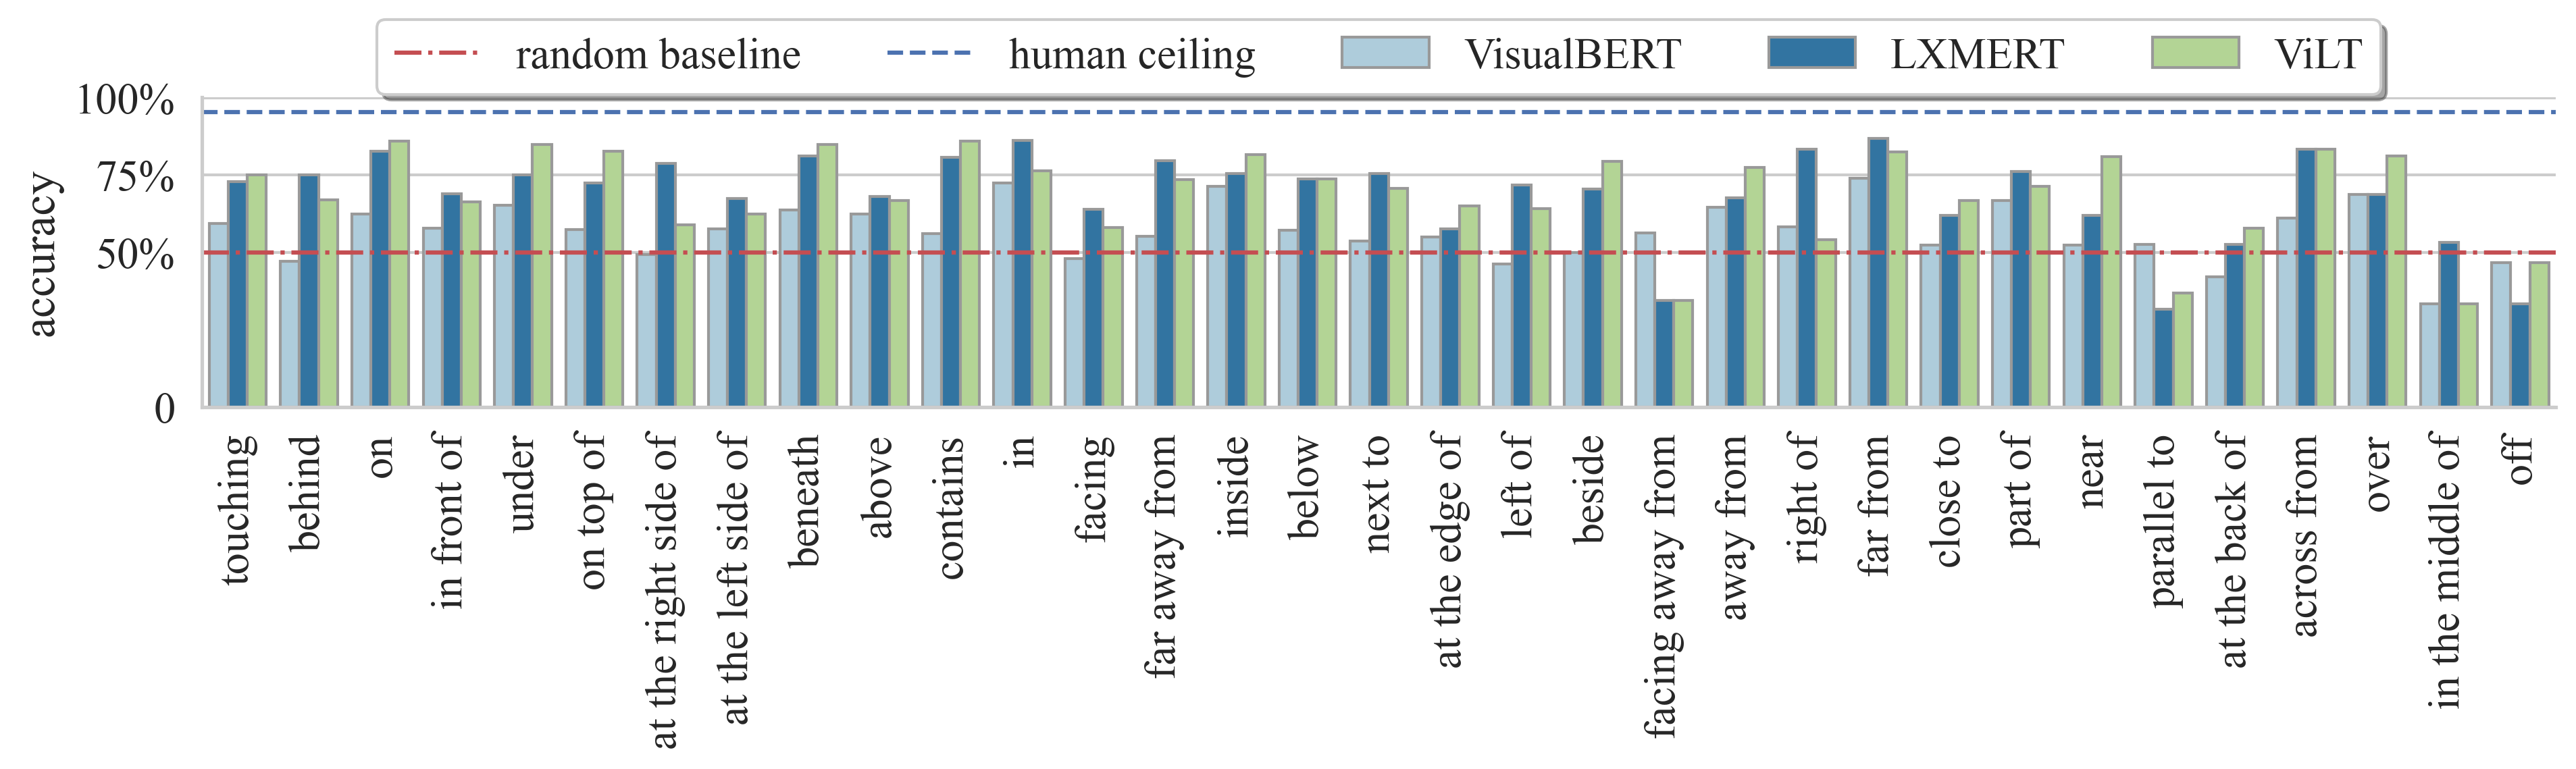
\includegraphics[width=\linewidth]{images/visual-spatial-reasoning/performance_by_relation_random_split_v2.png}
    \vspace{-1cm}
    \caption{random split}
\end{subfigure}
\begin{subfigure}[b]{\linewidth}
    \centering
    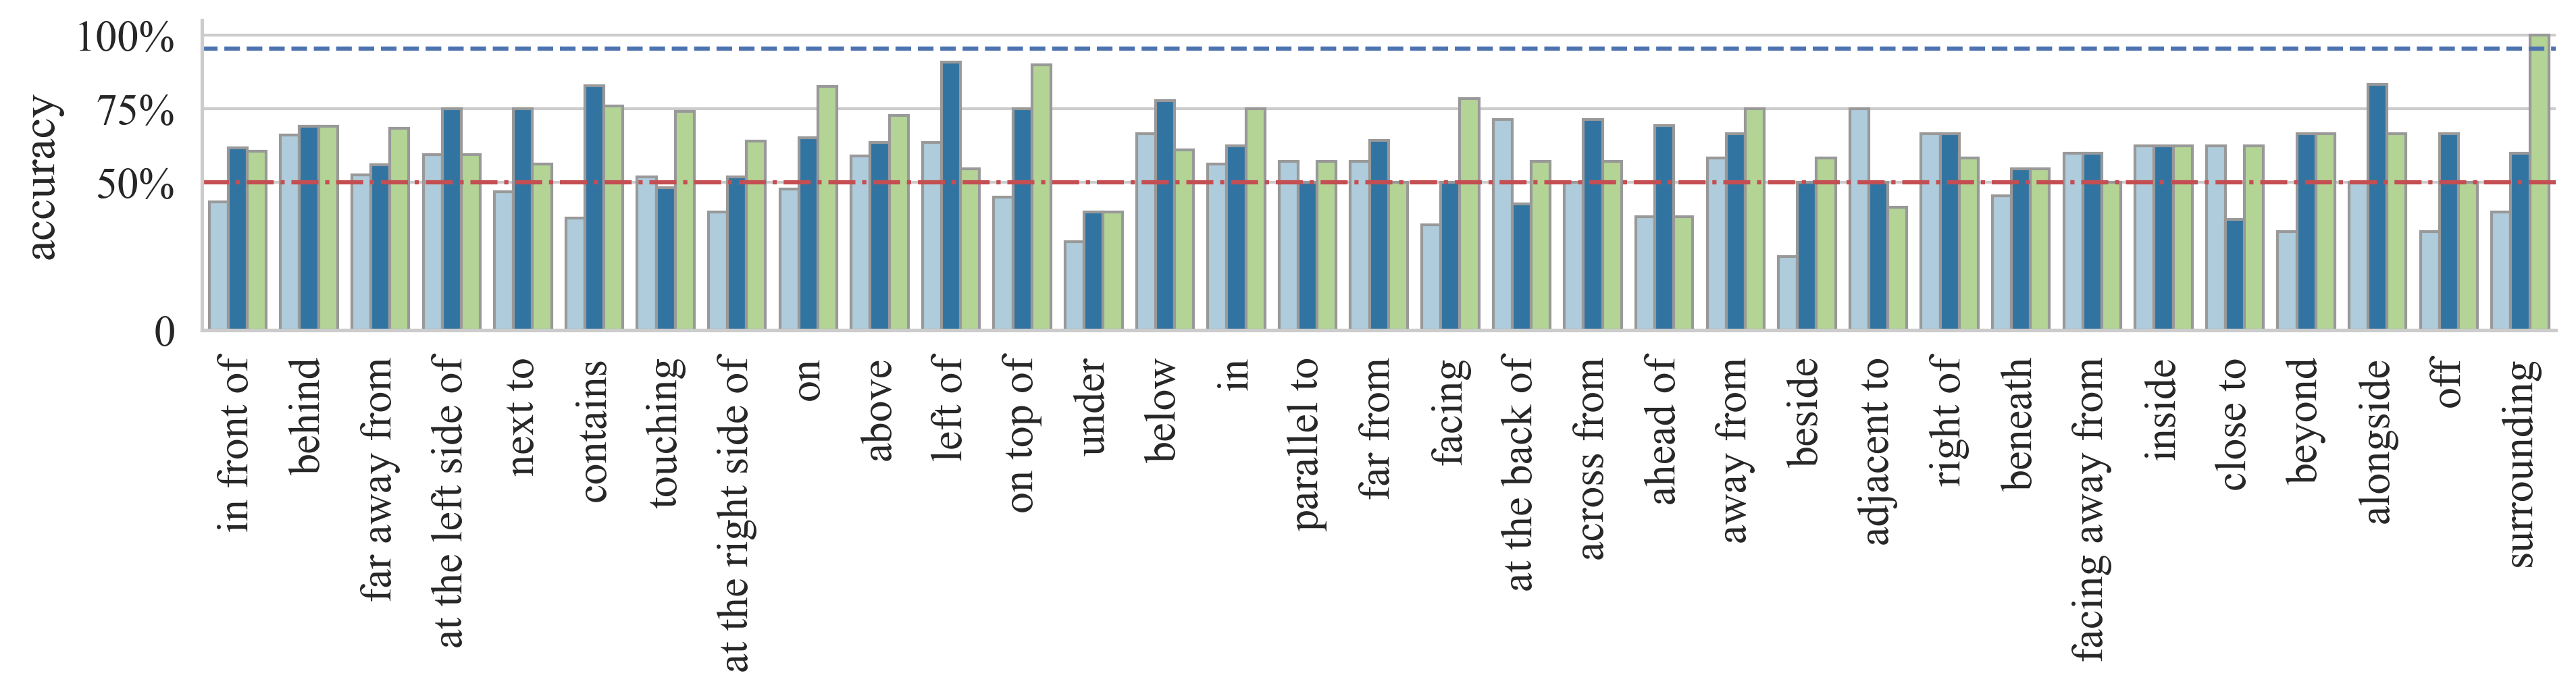
\includegraphics[width=\linewidth]{images/visual-spatial-reasoning/performance_by_relation_zeroshot_split_v2.png}
    \vspace{-1cm}
    \caption{zero-shot split}
\end{subfigure}
\caption{Performance by relation on the random (upper) and zero-shot (lower) split test sets. Relation order sorted by frequency (high to low from left to right). Only relations with more than 15 and 5 occurrences on the random and zero-shot tests respectively are shown. }
    \label{fig:performance_by_rel_base}
\end{figure*}

\subsubsection{Ours}

See \cref{fig:performance_by_rel}

\begin{figure}[ht]
    \centering
\begin{subfigure}[b]{\linewidth}
    \centering
    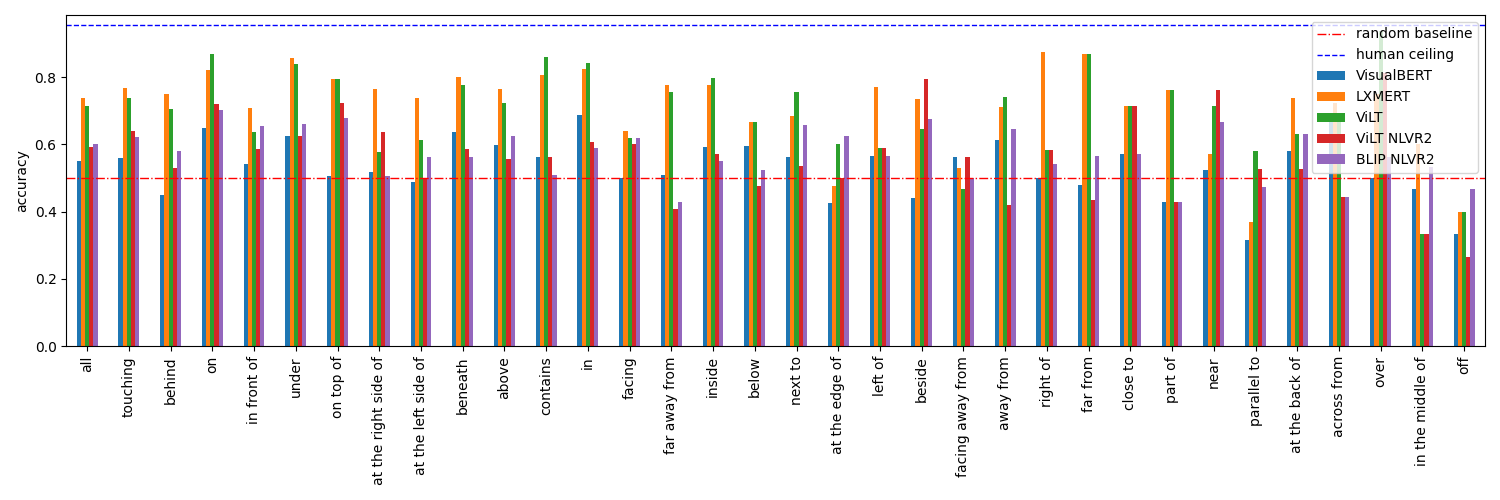
\includegraphics[width=\linewidth]{images/visual-spatial-reasoning/performance_rel_random.png}
    \vspace{-1cm}
    \caption{random split}
\end{subfigure}
\begin{subfigure}[b]{\linewidth}
    \centering
    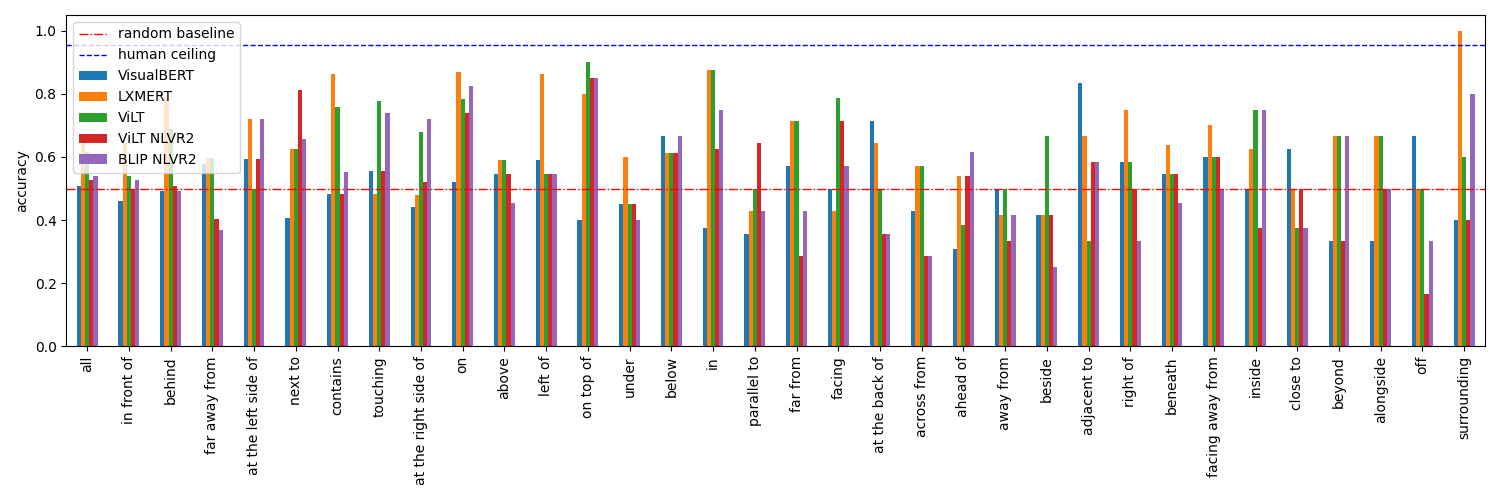
\includegraphics[width=\linewidth]{images/visual-spatial-reasoning/performance_rel_zeroshot.png}
    \vspace{-1cm}
    \caption{zero-shot split}
\end{subfigure}
\caption{Performance by relation on the random (upper) and zero-shot (lower) split test sets. Relation order sorted by frequency (high to low from left to right). Only relations with more than 15 and 5 occurrences on the random and zero-shot tests respectively are shown. }
    \label{fig:performance_by_rel}
\end{figure}

See \cref{tab:results-by-relation-random} and \cref{tab:results-by-relation-zeroshot}

\begin{table}[ht]
\centering
\begin{tabular}{lrrrrrr}
\toprule
relation &  number &  VisualBERT &  LXMERT &  ViLT &  ViLT NLVR2 &  BLIP NLVR2 \\
\midrule
all                  &    2024 &        55.1 &    73.9 &  71.2 &        59.1 &        60.1 \\
\midrule
touching             &     236 &        55.9 &    76.7 &  73.7 &        64.0 &        62.3 \\
behind               &     136 &        44.9 &    75.0 &  70.6 &        52.9 &        58.1 \\
on                   &     128 &        64.8 &    82.0 &  86.7 &        71.9 &        70.3 \\
in front of          &     116 &        54.3 &    70.7 &  63.8 &        58.6 &        65.5 \\
under                &     112 &        62.5 &    85.7 &  83.9 &        62.5 &        66.1 \\
on top of            &      87 &        50.6 &    79.3 &  79.3 &        72.4 &        67.8 \\
at the right side of &      85 &        51.8 &    76.5 &  57.6 &        63.5 &        50.6 \\
at the left side of  &      80 &        48.8 &    73.8 &  61.3 &        50.0 &        56.2 \\
beneath              &      80 &        63.7 &    80.0 &  77.5 &        58.8 &        56.2 \\
above                &      72 &        59.7 &    76.4 &  72.2 &        55.6 &        62.5 \\
contains             &      57 &        56.1 &    80.7 &  86.0 &        56.1 &        50.9 \\
in                   &      51 &        68.6 &    82.4 &  84.3 &        60.8 &        58.8 \\
facing               &      50 &        50.0 &    64.0 &  62.0 &        60.0 &        62.0 \\
far away from        &      49 &        51.0 &    77.6 &  75.5 &        40.8 &        42.9 \\
inside               &      49 &        59.2 &    77.6 &  79.6 &        57.1 &        55.1 \\
below                &      42 &        59.5 &    66.7 &  66.7 &        47.6 &        52.4 \\
next to              &      41 &        56.1 &    68.3 &  75.6 &        53.7 &        65.9 \\
at the edge of       &      40 &        42.5 &    47.5 &  60.0 &        50.0 &        62.5 \\
left of              &      39 &        56.4 &    76.9 &  59.0 &        59.0 &        56.4 \\
beside               &      34 &        44.1 &    73.5 &  64.7 &        79.4 &        67.6 \\
facing away from     &      32 &        56.2 &    53.1 &  46.9 &        56.2 &        50.0 \\
away from            &      31 &        61.3 &    71.0 &  74.2 &        41.9 &        64.5 \\
right of             &      24 &        50.0 &    87.5 &  58.3 &        58.3 &        54.2 \\
far from             &      23 &        47.8 &    87.0 &  87.0 &        43.5 &        56.5 \\
close to             &      21 &        57.1 &    71.4 &  71.4 &        71.4 &        57.1 \\
part of              &      21 &        42.9 &    76.2 &  76.2 &        42.9 &        42.9 \\
near                 &      21 &        52.4 &    57.1 &  71.4 &        76.2 &        66.7 \\
parallel to          &      19 &        31.6 &    36.8 &  57.9 &        52.6 &        47.4 \\
at the back of       &      19 &        57.9 &    73.7 &  63.2 &        52.6 &        63.2 \\
across from          &      18 &        66.7 &    72.2 &  66.7 &        44.4 &        44.4 \\
over                 &      16 &        50.0 &    75.0 &  93.8 &        81.2 &        56.2 \\
in the middle of     &      15 &        46.7 &    60.0 &  33.3 &        33.3 &        53.3 \\
off                  &      15 &        33.3 &    40.0 &  40.0 &        26.7 &        46.7 \\
\bottomrule
\end{tabular}
\caption{Number and performance by relation on the random split test. Only relations with more than 15 occurrences are shown.}
\label{tab:results-by-relation-random}
\end{table}

\begin{table}[ht]
\centering
\begin{tabular}{lrrrrrr}
\toprule
relation &  number &  VisualBERT &  LXMERT &  ViLT &  ViLT NLVR2 &  BLIP NLVR2 \\
\midrule
all                  &     731 &        50.8 &    65.5 &  61.6 &        52.8 &        53.9 \\
\midrule
in front of          &      76 &        46.1 &    64.5 &  53.9 &        50.0 &        52.6 \\
behind               &      71 &        49.3 &    78.9 &  69.0 &        50.7 &        49.3 \\
far away from        &      57 &        57.9 &    59.6 &  59.6 &        40.4 &        36.8 \\
at the left side of  &      32 &        59.4 &    71.9 &  50.0 &        59.4 &        71.9 \\
next to              &      32 &        40.6 &    62.5 &  62.5 &        81.2 &        65.6 \\
contains             &      29 &        48.3 &    86.2 &  75.9 &        48.3 &        55.2 \\
touching             &      27 &        55.6 &    48.1 &  77.8 &        55.6 &        74.1 \\
at the right side of &      25 &        44.0 &    48.0 &  68.0 &        52.0 &        72.0 \\
on                   &      23 &        52.2 &    87.0 &  78.3 &        73.9 &        82.6 \\
above                &      22 &        54.5 &    59.1 &  59.1 &        54.5 &        45.5 \\
left of              &      22 &        59.1 &    86.4 &  54.5 &        54.5 &        54.5 \\
on top of            &      20 &        40.0 &    80.0 &  90.0 &        85.0 &        85.0 \\
under                &      20 &        45.0 &    60.0 &  45.0 &        45.0 &        40.0 \\
below                &      18 &        66.7 &    61.1 &  61.1 &        61.1 &        66.7 \\
in                   &      16 &        37.5 &    87.5 &  87.5 &        62.5 &        75.0 \\
parallel to          &      14 &        35.7 &    42.9 &  50.0 &        64.3 &        42.9 \\
far from             &      14 &        57.1 &    71.4 &  71.4 &        28.6 &        42.9 \\
facing               &      14 &        50.0 &    42.9 &  78.6 &        71.4 &        57.1 \\
at the back of       &      14 &        71.4 &    64.3 &  50.0 &        35.7 &        35.7 \\
across from          &      14 &        42.9 &    57.1 &  57.1 &        28.6 &        28.6 \\
ahead of             &      13 &        30.8 &    53.8 &  38.5 &        53.8 &        61.5 \\
away from            &      12 &        50.0 &    41.7 &  50.0 &        33.3 &        41.7 \\
beside               &      12 &        41.7 &    41.7 &  66.7 &        41.7 &        25.0 \\
adjacent to          &      12 &        83.3 &    66.7 &  33.3 &        58.3 &        58.3 \\
right of             &      12 &        58.3 &    75.0 &  58.3 &        50.0 &        33.3 \\
beneath              &      11 &        54.5 &    63.6 &  54.5 &        54.5 &        45.5 \\
facing away from     &      10 &        60.0 &    70.0 &  60.0 &        60.0 &        50.0 \\
inside               &       8 &        50.0 &    62.5 &  75.0 &        37.5 &        75.0 \\
close to             &       8 &        62.5 &    50.0 &  37.5 &        50.0 &        37.5 \\
beyond               &       6 &        33.3 &    66.7 &  66.7 &        33.3 &        66.7 \\
alongside            &       6 &        33.3 &    66.7 &  66.7 &        50.0 &        50.0 \\
off                  &       6 &        66.7 &    50.0 &  50.0 &        16.7 &        33.3 \\
surrounding          &       5 &        40.0 &   100.0 &  60.0 &        40.0 &        80.0 \\
\bottomrule
\end{tabular}
\caption{Number and performance by relation on the zero-shot split test. Only relations with more than 5 occurrences are shown.}
\label{tab:results-by-relation-zeroshot}
\end{table}

\subsection{Results By Relation Meta Category}

\subsubsection{Baseline}

See \cref{fig:performance_by_meta_cat_base}

\begin{figure*}
    \centering
\begin{subfigure}[b]{0.49\linewidth}
    \centering
    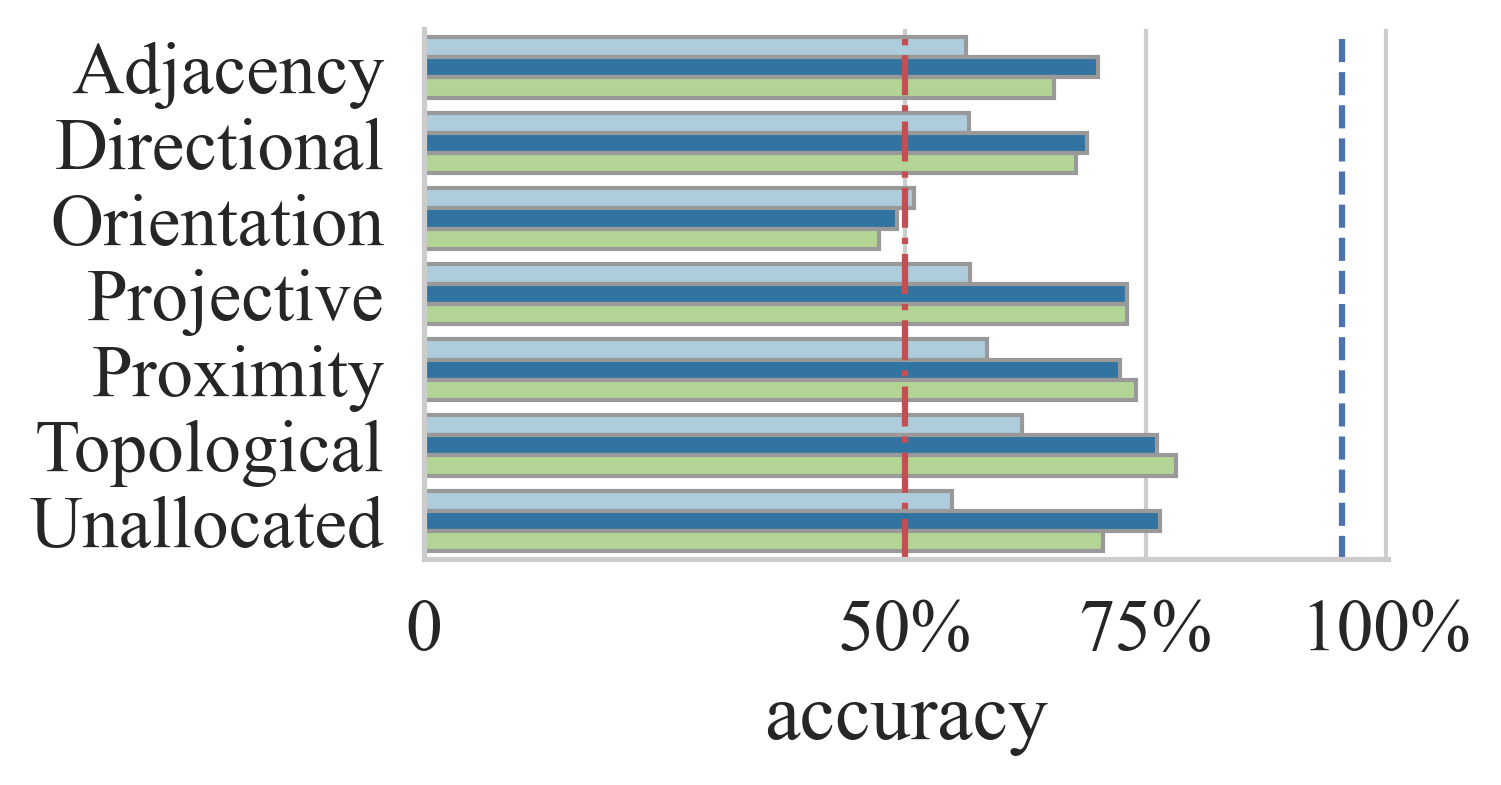
\includegraphics[width=\linewidth]{images/visual-spatial-reasoning/performance_by_meta_cat_random_split_v2.png}
    \caption{random split}
\end{subfigure}
\begin{subfigure}[b]{0.49\linewidth}
    \centering
    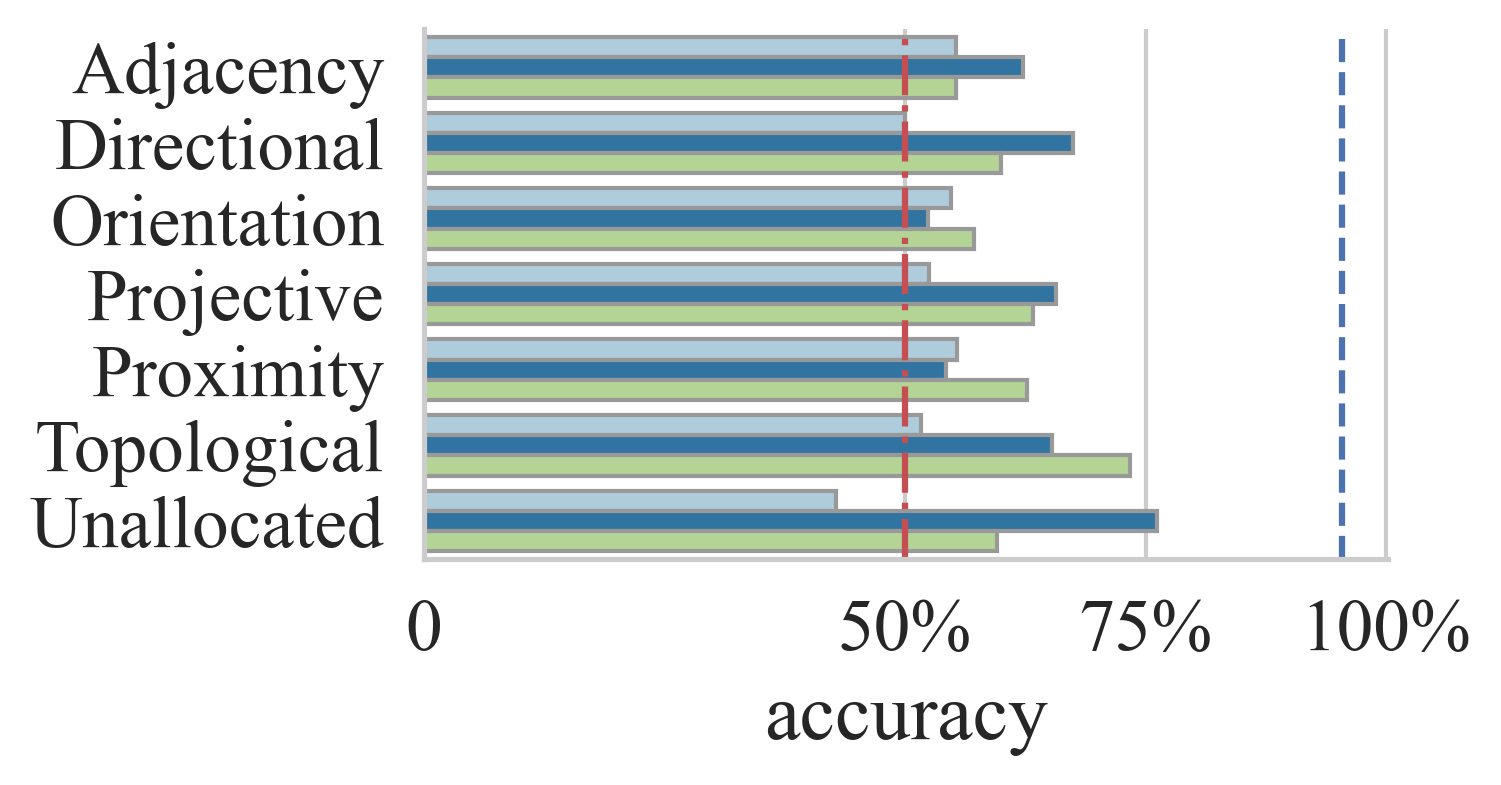
\includegraphics[width=\linewidth]{images/visual-spatial-reasoning/performance_by_meta_cat_zeroshot_split_v2.png}
    \caption{zero-shot split}
\end{subfigure}
\caption{Performance by meta categories of relations, on the random (left) and zero-shot (right) split test sets. For legend information, see \Cref{fig:performance_by_rel_base}.}
    \label{fig:performance_by_meta_cat_base}
\end{figure*}

\subsubsection{Ours}

See \cref{fig:performance_by_meta_cat}

\begin{figure}[ht]
    \centering
    \begin{subfigure}[b]{0.49\linewidth}
    \centering
    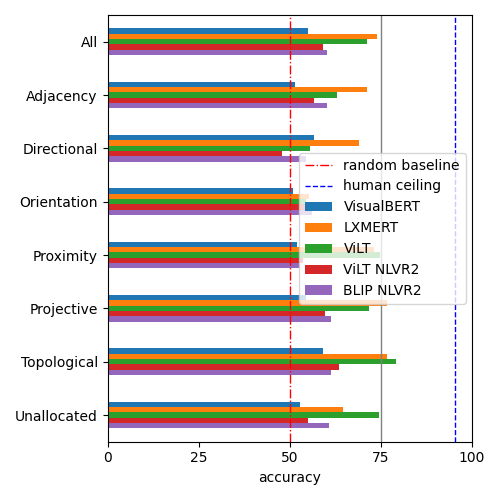
\includegraphics[width=\linewidth]{images/visual-spatial-reasoning/performance_rel_meta_cat_random.png}
    \caption{random split}
     \end{subfigure}
     \begin{subfigure}[b]{0.49\linewidth}
         \centering
    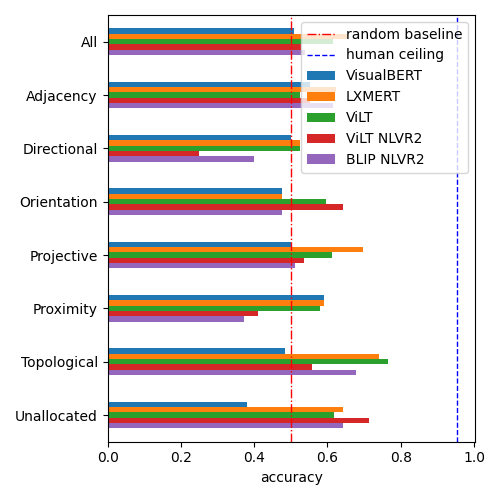
\includegraphics[width=\linewidth]{images/visual-spatial-reasoning/performance_rel_meta_cat_zeroshot.png}
         \caption{zero-shot split}
     \end{subfigure}
\caption{Performance by meta categories of relations, on the random (left) and zero-shot (right) split test sets. For legend information, see \cref{fig:performance_by_rel}.}
    \label{fig:performance_by_meta_cat}
\end{figure}

See \cref{tab:results-by-relation-meta-category-random} and \cref{tab:results-by-relation-meta-category-zeroshot}

\begin{table}[ht]
\centering
\begin{tabular}{lrrrrrr}
\toprule
category &  number &  VisualBERT &  LXMERT &  ViLT &  ViLT NLVR2 &  BLIP NLVR2 \\
\midrule
All         &    2024 &        55.1 &    73.9 &  71.2 &        59.1 &        60.1 \\
\midrule
Adjacency   &     284 &        51.4 &    71.1 &  63.0 &        56.7 &        60.2 \\
Directional &      90 &        56.7 &    68.9 &  55.6 &        47.8 &        54.4 \\
Orientation &     112 &        50.9 &    55.4 &  54.5 &        55.4 &        56.2 \\
Proximity   &     123 &        52.0 &    73.2 &  74.8 &        53.7 &        52.8 \\
Projective  &     773 &        54.5 &    76.7 &  71.7 &        59.8 &        61.4 \\
Topological &     591 &        59.2 &    76.8 &  79.2 &        63.5 &        61.4 \\
Unallocated &      51 &        52.9 &    64.7 &  74.5 &        54.9 &        60.8 \\
\bottomrule
\end{tabular}
\caption{Number and performance by relation meta category on the random split test.}
\label{tab:results-by-relation-meta-category-random}
\end{table}

\begin{table}[ht]
\centering
\begin{tabular}{lrrrrrr}
\toprule
category &  number &  VisualBERT &  LXMERT &  ViLT &  ViLT NLVR2 &  BLIP NLVR2 \\
\midrule
All         &     731 &        50.8 &    65.5 &  61.6 &        52.8 &        53.9 \\
\midrule
Adjacency   &     114 &        55.3 &    62.3 &  52.6 &        55.3 &        61.4 \\
Directional &      40 &        50.0 &    52.5 &  52.5 &        25.0 &        40.0 \\
Orientation &      42 &        47.6 &    47.6 &  59.5 &        64.3 &        47.6 \\
Proximity   &      83 &        59.0 &    59.0 &  57.8 &        41.0 &        37.3 \\
Projective  &     286 &        50.0 &    69.6 &  61.2 &        53.5 &        51.0 \\
Topological &     124 &        48.4 &    74.2 &  76.6 &        55.6 &        67.7 \\
Unallocated &      42 &        38.1 &    64.3 &  61.9 &        71.4 &        64.3 \\
\bottomrule
\end{tabular}
\caption{Number and performance by relation meta category on the zero-shot split test.}
\label{tab:results-by-relation-meta-category-zeroshot}
\end{table}
